\chapter{Redox activity of Single-azurin at diffferent electrochemical potential}
\section{Introduction}
\section{Experimental Method}
\section{Results and Discussion}
\section{Results and discussion\label{sec:results}}
%Scheme
\begin{scheme}
	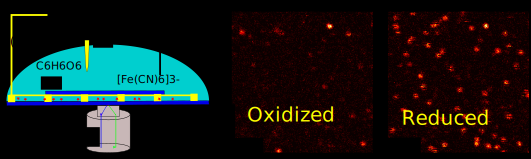
\includegraphics[scale=0.5]{Figure/Scheme_1_setup.eps}
	\caption{The scheme picture of the final setup. \textbf{(1)}  Objective through which light is irradiated on and collected from the sample. \textbf{(2)} The functionalized sample slide with on top the platinum grid
and another small glass slide to press the grid on the sample slide, resulting in small confined volumes in the order of nanoliters. \textbf{(3)} The electron mediator solution consisting of 200 μM ferricyanide, 100 μM ascorbate in PBS (PH 7.4) buffer with a total volume of 4 mL. \textbf{(4)} The working electrode (Platinum wire) that is in contact with the platinum grid. \textbf{(5)} The saturated calomel reference electrode. \textbf{(6)} The Platinum wire (not touching the grid) as counter electrode. \textbf{(7)} The potentiostat (Model 800B Series Electrochemical Detector, CH Instruments) to which the electrodes are connected. \textbf{(8)}, \textbf{(9)} Top view of the sample slide and two images are showing the labeled Cu-Azurin reduced(brighter) and oxidized(dimmer).}
  	\label{sch:setup}
\end{scheme}
%time trace
\begin{figure}
	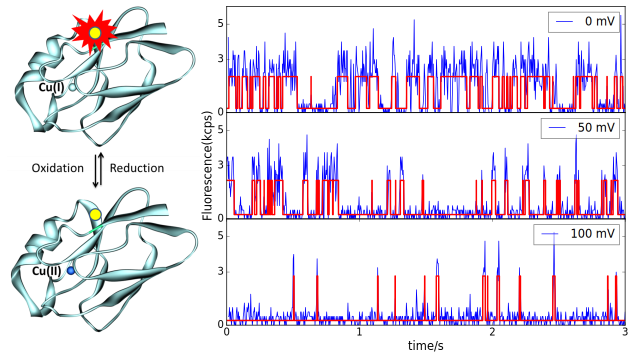
\includegraphics[width=\textwidth]{Figure/Figure_1_timetrace_CuAzu.eps}
	\caption{Time traces of Cu-Azurin labeled with ATTO655 at different potentials. The structure of the protein with properly positioned dye can be seen in the schematic picture in the left. In Cu(II) state (shown in bluish atom in the protein structure), the dye is non fluorescent because of FRET and in Cu(I) state (shown in gray atom), the dye is fluorescent. Notice the amount of time the protein spends on bright and dark state at different potentials. At lower potentials (e.g 0 mV) the protein is brighter most of the time because of the higher concentration of reductant.}
	\label{fig:timetrace}
\end{figure}
%Midpoint histogram
\begin{figure}
	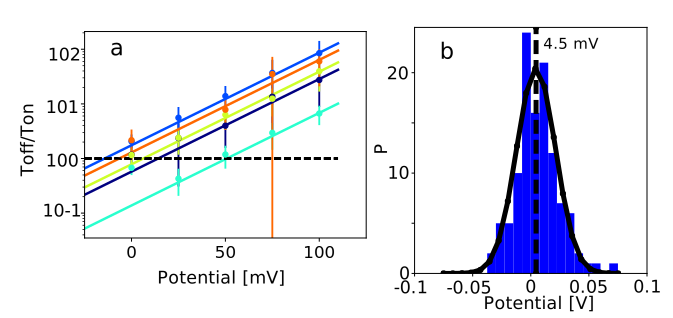
\includegraphics[width=\textwidth]{Figure/Figure_2_midpoint.eps}
	\caption{Ratio between on and off time as a function of applied potential for the same single-molecule. Different color represents different single-molecules. And the line connecting the data points is the Nernst fit for all the data points above 25 mV. The plot in the right is the histogram of midpoint potentials for $132$ molecules with a gaussian fit with center 4.5 mV with respect to calomel electrode.}
	\label{fig:midpoint}
\end{figure}
%on-off 1D histogram
\begin{figure}
	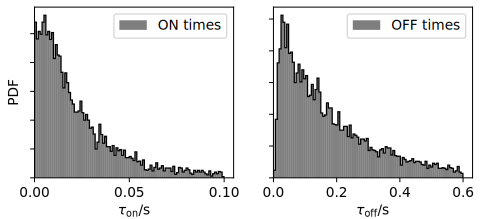
\includegraphics[width=\textwidth]{Figure/Figure_3_on_off_1D.eps}
	\caption{\textbf{On off histogram.} The histogram of on-times(a) and of off-times(b) of Cu-Azurin-ATTO655 showing rise time. This indicates that both oxidation and reduction of Cu-Azurin occurs through an intermediate step.}
	\label{fig:onoff1D}
\end{figure}
%on-off 2D histogram
\begin{figure}
	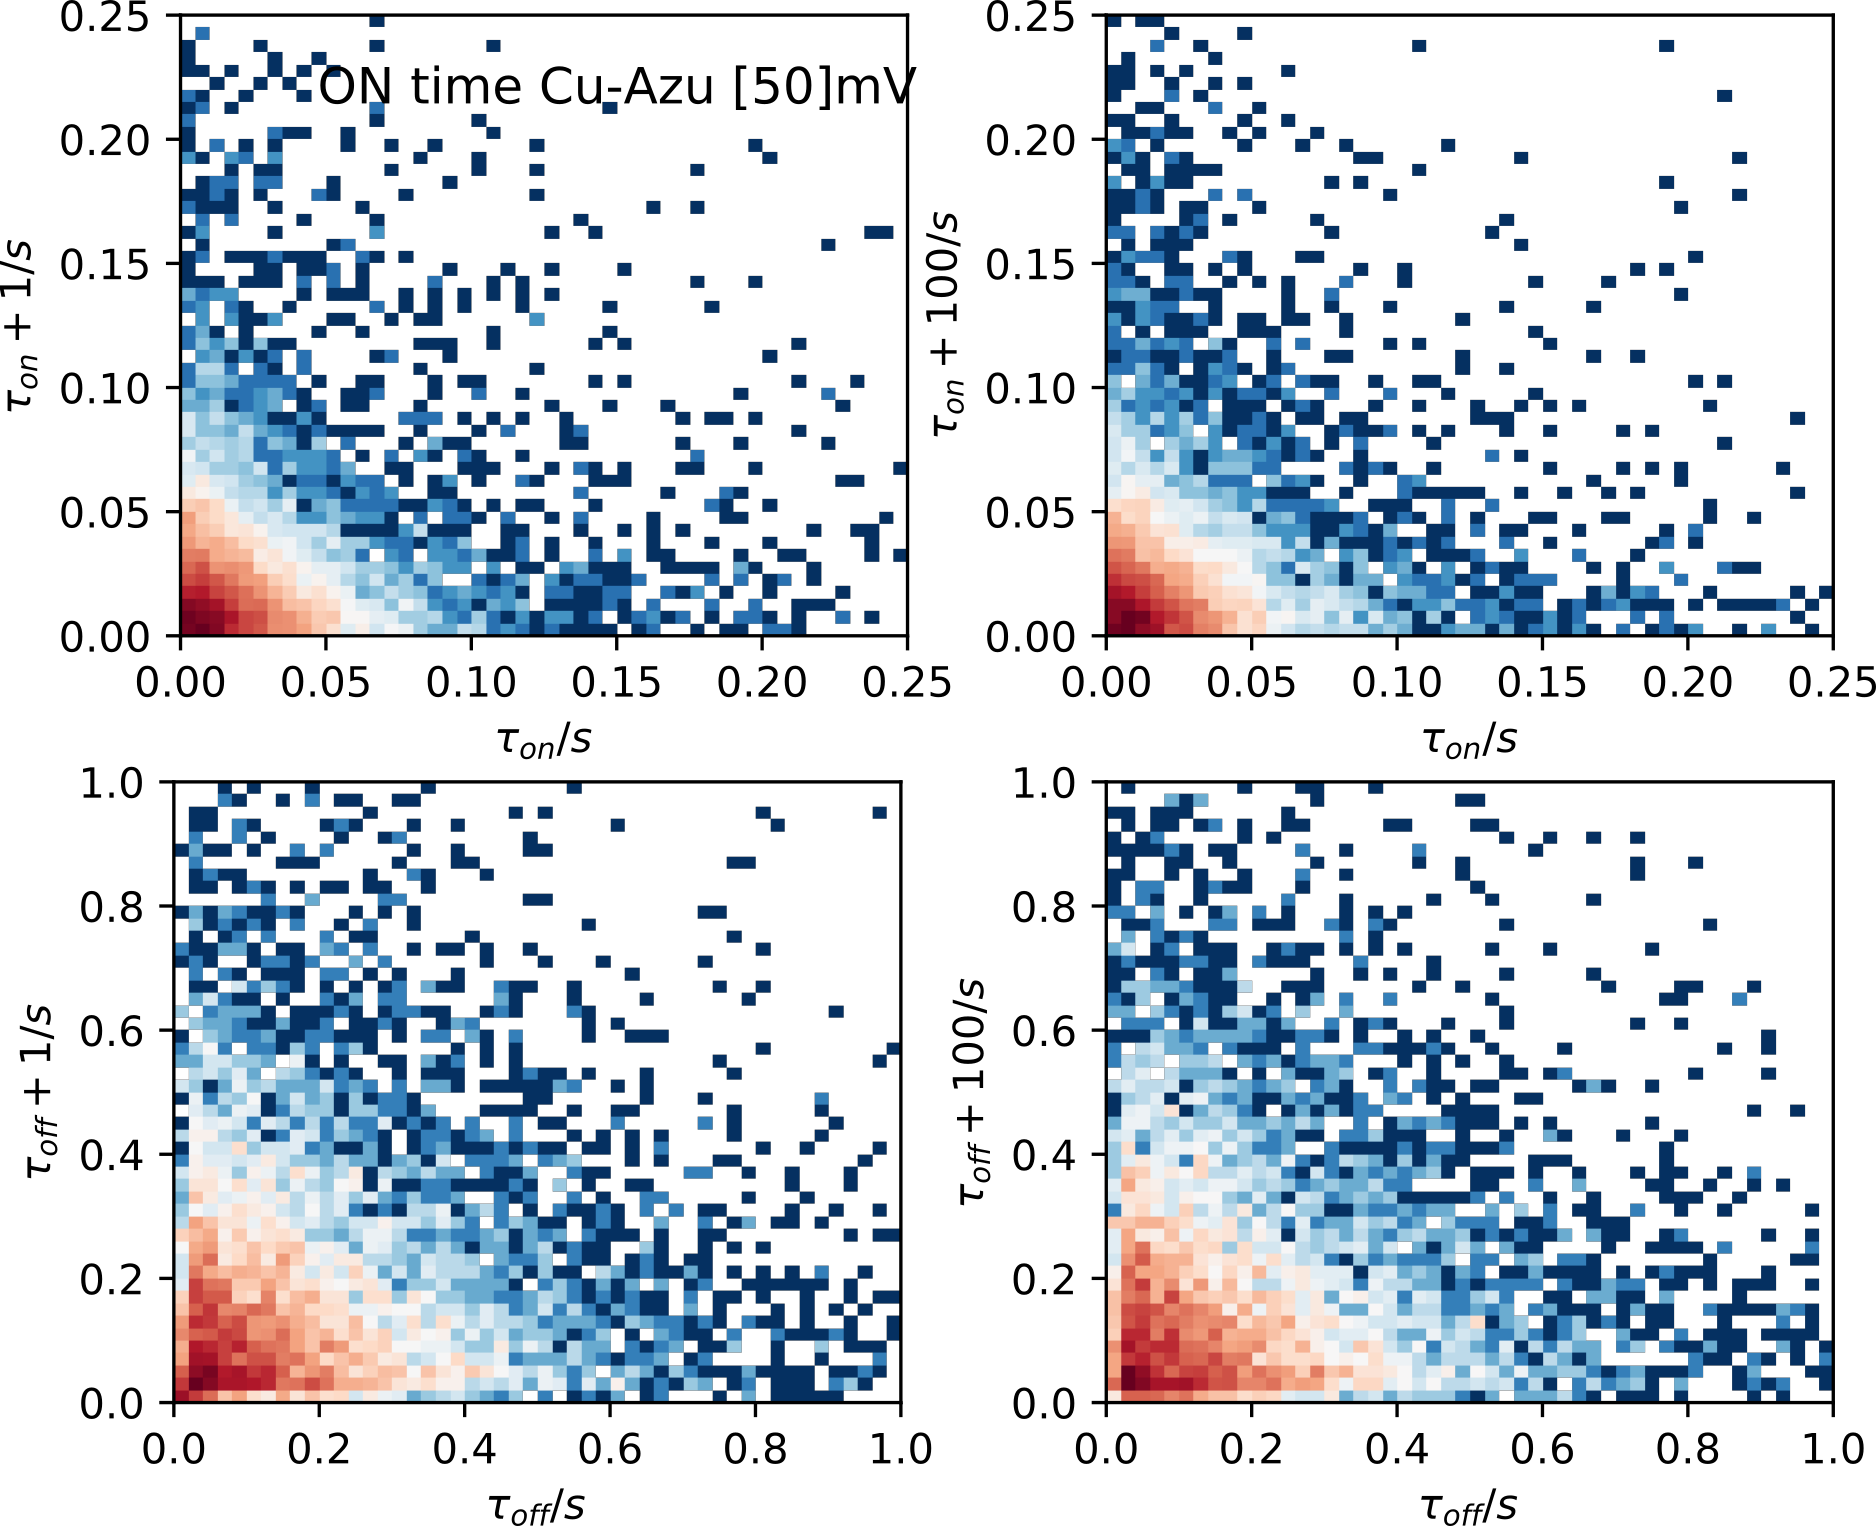
\includegraphics[width=\textwidth]{Figure/Figure_4_on_off_2D_100mV.png}
	\caption{\textbf{2D histogram: Cu-Azurin.} 2D correlation plot of (a) on-times vs the next on-times (b) on-times vs the on-time after 100 turnovers (c) off-times vs next off-times (d) off-times vs the off-time after 100 turnovers.}
	\label{fig:onoff2D}
\end{figure}
\subsection{Ensemble fluorescence switching}
\subsection{Single-molecule switching}
\subsection{Active and inactive periods in enzymatic activity}
\section{Conclusion}